\documentclass[tikz]{article}
\usepackage[left=1.8cm,right=3cm,top=1.5cm,bottom=2cm]{geometry} % page
% settings
\usepackage{multicol} 
\usepackage{amsmath} % provides many mathematical environments & tools
\usepackage{dsfont}
\usepackage{upgreek}
\usepackage[english]{babel}
\usepackage[doument]{ragged2e}

\usepackage{tikz}
\tikzset{
  every point/.style = {radius={\pgflinewidth}, opacity=1, draw, solid, fill=white},
  pt/.pic = {
    \begin{pgfonlayer}{foreground}
      \path[every point, #1] circle;
    \end{pgfonlayer}
  },
  point/.style={insert path={pic{pt={#1}}}}, point/.default={},
  colored point/.style = {point={fill=#1}},
  point name/.style = {insert path={coordinate (#1)}}
}

% Images
\usepackage{graphicx}
\usepackage{float}
\usepackage{subfigure} % subfiguras
\usepackage{caption}
\captionsetup[table]{labelformat=empty}
\captionsetup[figure]{labelformat=empty}

\usepackage{listings}
\usepackage{xcolor}
\definecolor{gray}{rgb}{0.5,0.5,0.5}
\newcommand{\n}[1]{{\color{gray}#1}}
\lstset{numbers=left,numberstyle=\small\color{gray}}

\selectlanguage{english}
\usepackage[utf8]{inputenc}
\setlength{\parindent}{0mm}

\begin{document}

\title{Ejercicios propuestos: Temas 1 y 2 (Parte II)}
\author{David Cabezas Berrido}
\date{}
\maketitle

\section*{Ejercicio 2}

Sea $(X,Y)$ un vector continuo con la función de densidad conjunta que
se muestra a continuación
\[f(x,y)=\frac{1}{64}, \quad -2<x<6,\ -2-x<y<x+2\]

Obtener la función de densidad de $y$ condicionada a un valor $x_0$,
así como la función de densidad de $x$ condicionada a un valor
$y_0$. A través de estas funciones de densidad condicionadas, calcular
$P(Y>1.34|X=1.97)$ y $P(X<1.97|Y=1.34)$.

\begin{center}
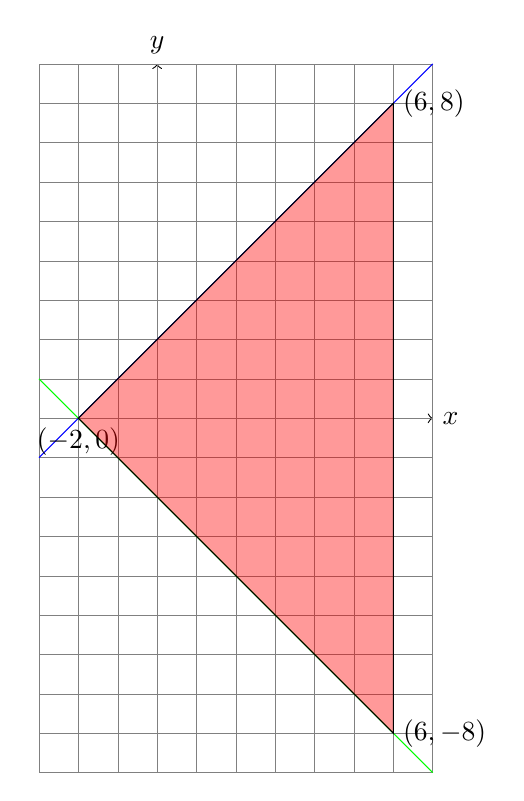
\begin{tikzpicture}[scale=0.5]

  \draw[->] (-3,0) -- (7,0) node[right] {$x$};
  \draw[->] (0,-9) -- (0,9) node[above] {$y$};

  \draw[style=help lines] (-3,-9) grid (7,9);
  
  \draw[domain=-3:7,smooth,variable=\x,blue] plot ({\x},{\x+2});
  \draw[domain=-3:7,smooth,variable=\x,green] plot ({\x},{-\x-2});

  \node at (-2,0) [below] {$(-2,0)$};
  \node at (6,-8) [right] {$(6,-8)$};
  \node at (6,8) [right] {$(6,8)$};

  \draw[fill=red, fill opacity=0.4] (-2,0) -- (6,-8) -- (6,8) -- cycle;
\end{tikzpicture}
\end{center}

\end{document}